
\documentclass[a4paper,lithuanian]{article}

\usepackage[utf8]{inputenc}
\usepackage[L7x]{fontenc}
\usepackage[lithuanian]{babel}
\usepackage{graphicx}
\graphicspath { {./} }

\title{MU5 Kompiuterio techninis aprašymas}

\author{
  Adam Jasinski\\
  VU MIF, Bioinformatika, II kursas
}

\begin{document}

\maketitle

\newpage

\section{Įvadas}

MU5 yra penktoji kompiuterio sistema suprojektuota ir pastatyta Mančesterio Universitete nuo 1946 metų. Ankstesni Mančesterio Universiteto darbai, ypač \\Manchester Mark 1 ir Atlas turėjo didelę reikšmę industrijoje ir moksle. Ankstesnės mašinos buvo sukurtos Elektrinės inžinerijos skyriaus nariais o 1964 metais, buvo suformuota atskira informatikos katedra, kurios tikslu buvo reikšminga mokslinės veiklos plėtra, pradedant pirmais informatikos absolventų metais. Tuo metu, universitetas naudojo anksčiau minėtą Atlas kaip skaičiavimų vykdymo sistemą, ir iš patirties buvo nuspręsta, kad aparatūros ir programinės įrangos vystymas negali būti efektyviai atliekamas naudojant viso universiteto eksploatuojamą skaičiavimų vykdymo sistemą. To rezultatu gimė reikmė nepriklausomai, specifinei įrangai katedros veiklai, bet taip pat noras tęsti pažangių sistemų projektavimą, statymą ir novatoriškų idėjų plėtojimą, kurios vėliau galėtų būti išnaudojamas kompiuterių industrijos.\newline

1968 sausį, po kelių metų diskusijų, MU5 projektui buvo suteikta £630.446 mokslinė stipendija, kurios pakako tik mažai versijai (architektūriniu mastu) potencialiai didelės sistemos. Fiziškai, MU5 buvo didelė mašina, ką galite pamatyti 1 pav.\newline



\begin{figure}[h]
	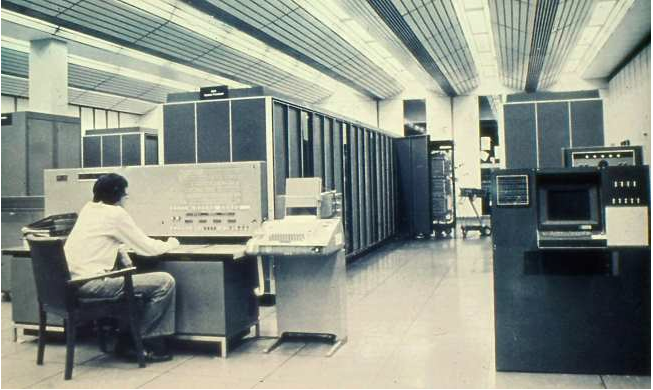
\includegraphics[scale=0.4]{mu5-room}
	\centering
	\caption{MU5 kambarys, su jo operatoriumi prie konsolės}
	\label{}
\end{figure}

MU5 paleidimo darbai prasidėjo 1971 vasarą, o pilnai veikti pradėjo 1974 vidury, kai atsirado galimybė leisti Algol ir Fortran programas. Praeiti Mančesterio Universiteto kūriniai turėjo tiesioginį komercinį atitikmenį, kai MU5 tokio neturėjo, užtat galėjo pasigirti didele įtaka ICL 2900 serijos kompiuterių architektūrai, kurioje operacijų kodas, adresavimo struktūra ir operandų formos skiriasi tik smulkmenomis nuo MU5. \newline

Pilnai veikiantis MU5 kompiuteris teikė skaičiavimų vykdymo paslaugą iki 25 aktyvių vartotojų vienu metu, iki kol nebuvo išrinktas 1982 metais.




\section{Dizaino idėjos}

MU5 pagrindinė idėja buvo tai, kad vidinė kompiuterio struktūra turi atvaizduoti struktūrą programų, kuriomis bus programuojama. Algol ir Fortran buvo dvi to laiko pagrindinės programavimo kalbos, iš kurių pirmoji išsiskyrė rekursija ir dinaminiu atminties priskyrimu, o kita programomis be rekursijos, su kompiliavimo metu priskiriama atmintimi, bet abi jos turėjo šias bendras charakteristikas:

\begin{itemize}
\item Kiekviena programa turi savo lokalinę darbo erdvę, sudarytą iš sveikųjų ir slankiojo kablelio duomenų tipų
\item Programa gali kreiptis į nelokalinius kintamuosius apgaubiamojoje programoje arba erdvėje bendroje visoms programoms
\item Deklaravimas gali apimti bet kokį operandų skaičių, kurie gali būti vardai, sveikųjų skaičių vardai, masyvo elementai, funkcijos kvietimai arba konstantos.
\end{itemize}

Vardų erdvės sąvoka yra viena pagrindinių idėjų MU5 dizaine. Standartiniuose kompiuteriuose, kintamieji paprastai būtų laikomi greituose, adresuojamuose bendros prieigos registruose. Tai yra tipinis pavyzdys 'pajėgiuose' kompiuteriuose, kur 'pajėgumas' pilnai išgaunamas iš aparatūros ar tai rankinio programavimo būdu ar kompleksinių ir daug laiko atimančių algoritmų naudojimas kompiliatoriuose. MU5 yra panaudotas sprendimas be paminėtų registrų, dažnai naudojami kintamieji yra laikomi greitoje asociatyviai adresuojamoje atmintyje. Instrukcijų formate yra informacija apie naudojamo operando tipą (skaliaras, vardas, konstanta, masyvo elementas ir t.t) kas leidžia procesoriui pasirinkti tik reikiamus kintamuosius buferizavimui vardų erdvėje, priešingai nei tradicinė 'cache' sistema, kuri buferizuoja blokus pagrindinės atminties neselektyviai. Tokiu būdu, paprastas, ciklinis žodžių keitimo algoritmas, ir jo palygintinas mažas dydis (448 bitai) leidžia gauti efektyvumą, panašų 'cache' sistemos. Tokiu būdu, kintamasis gali būti perrašomas daugybę kartų vardų erdvėje, bet pati vardų erdvė yra atnaujinama tik tada, kai eilutė su kintamuoju yra išrinkta keitimui. 

\section {Registrai}

MU5 turėjo penkis akumuliatorius, arba stekus. Kiekvienas iš jų galėjo akumuliuoti savo turinį, MU5 reikšmingu skirtumu buvo tai, kad kiekvieno iš šių stekų viršutiniai žodžiai buvo pasiekiami 'skaičiavimo registruose'. Kiekvienas iš registrų turėjo specifinę rolę ir jie yra išsklaidyti arti prie atitinkamų aritmetinių vienetų susijusių su ta funkcija. 
\begin{itemize}
\item Vienetas B - skirtas indeksų aritmetikai ir ciklų skaičiavimui
\item Vienetas D - skirtas adresų modifikacijai ir ribų tikrinimui
\item Vienetas A - pagrindinis aritmetinis vienetas skirtas sveikųjų, slankiojo kablelio ir dešimtainių skaičių skaičiavimui
\end{itemize}
O registrai yra 
\begin{itemize}
\item B   - 32 bitų modifikuojantis registras
\item DR  - 64 bitų registras vektorių deskriptoriams
\item XDR - panašus į DR ir naudojamas žodžių pernešimo instrukcijoms
\item X   - 32 bitų fiksuoto kablelio registras A vienete
\item ACC - 64 bitų registras A vienete   
\end{itemize}
MU5 vardų erdvė yra sudaryta iš 32 asociatyvių registrų, savyje turinčių kintamųjų adresus, ir 32 registrus, turinčius atitinkamas 'values'

\section {Adresavimas}

MU5 naudojo virtualų adresavimo režimą. To priežastimi buvo tai, kad pagrindinė operacinės sistemos užduotis yra vardų erdvės valdymas, kurio dominuojanti dalis buvo susijusi su automatiniu informacijos judėjimu tarp atminties lygių. Toks judėjimas reikalauja tikrųjų informacijos adresų judėjimas, jeigu šiems adresams bus leista išsisklaidyti po programos atmintį, tai gali privesti prie tam tikrų problemų. Pabaigoje buvo nutarta naudoti didelį virtualų adresą ir padalinti jį į tam tikrą segmentų skaičių. Adresas yra dalinamas į tris laukus, 4 bitų proceso numeris, 14 bitų segmento skaičius ir 16 bitų adresas apibrėžiantis 32 bitų žodį segmento viduje.

\newpage

\section {Mikroarchitektūra}

Svarbiausia MU5 procesoriaus mikroarchitektūros dalis yra pagrindinis operandų vienetas (Primary Operand Unit (PROP)) kuriam buvo tiekiamos instrukcijos iš instrukcijų buferio vieneto (IBU), o virtualių į tikruosius adresus konversija vyko talpyklos prieigos kontrolės vienete (Store Access Control Unit (SAC)), kuris koordinavo užklausas lokaliai talpyklai. Prieiga prie antrinių operandų vieneto naudojant deskriptorių mechanizmą reikalavo dviejų logiškai skirtingų dalių, viena adresų formavimui (Descriptor Addressing Unit) ir viena operandų pasirinkimui iš atitinkamo šiuo metu laikomo žodžio (Descriptor Operand Processing Unit), kartu su operandų buferio sistema (Operand Buffer System) kuri buvo įdiegta tarp jų, formuojant antrinį operandų vienetą (Secondary Operand Unit (SEOP)) Akumuliatoriaus vienetas (turintis iš esmės slankiojo kablelio vykdymo įrangą) akivaizdžiai turėjo būti įdiegtas už SEOP, nes didžiąją dalį laiko dorotų masyvų elementus, kuriuos priėjo SEOP, kitoje pusėje B vienetas buvo įdiegtas arčiau PROP, paraleliai su deskriptorių adresavimo vienetu, nes jis turėjo pateikti modifikavimo reikšmes, todėl daugiausiai dirbtų su įvardytais kiekiais, o ne masyvo elementais.

\begin{figure}[h]
	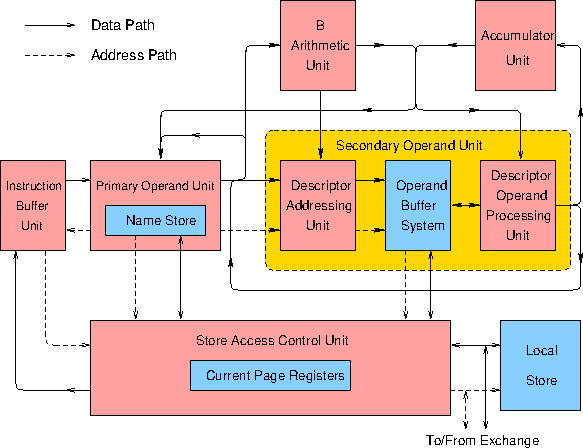
\includegraphics[scale=0.4]{mu5-march}
	\centering
	\caption{MU5 mikroarchitektūra}
	\label{}
\end{figure}

\section {Architektūros instrukcijų rinkinys}

\begin{center}
\begin{tabular}{||c c||||c c||} 
\multicolumn{4} {|c|}{B ir ACC} \\
 \hline
 Instrukcija & Veiksmas & Instrukcija & Veiksmas\\ [0.5ex] 
 \hline\hline
 LD & B = OP & LD & ACC = OP\\ 
 LDD & B = OP - 1 & SLD & Stack OP ACC = OP \\
 SLD & Stack OP B = OP & ST & ACC => OP \\
 ST & B => OP & ADD & ACC + OP \\ [1ex]
 ADD & B + OP & SUB & ACC - OP\\ [1ex] 
 SUB & B - OP & MUL & ACC * OP \\
 MUL & B * OP & DIV & ACC / OP\\
 XOR & B xor OP & XOR & B xor OP\\
 \hline
\end{tabular}
\end{center}

\section {

\newpage


\begin{thebibliography}{9}
\bibitem{mu5system}
Morris, D., Ibbett, R. (1979). The MU5 Computer System (MacMillan Computer Science). Palgrave HE UK.

\bibitem{devMU5}
Ibbett, R. N.; Capon, P. C. (1978). The development of the MU5 computer system.London

\bibitem{structure}
D. Morris, G. D. Detlefsen, G. R. Frank, T. J. Sweeney, The Structure of the MU5 Operating System, The Computer Journal, Volume 15, Issue 2, May 1972, Pages 113–116, https://doi.org/10.1093/comjnl/15.2.113
\end{thebibliography}

\end{document}
